% Generated by tools/rbq_fig_*.py from committed records. Do not edit by
% hand: regenerate instead, so the figure and its manifest entry stay in
% step. Records read are listed in
% experiments/mmsys2027_rbq_retarget_20260914/paper_figures_20260915/FIGURES_R1.json.
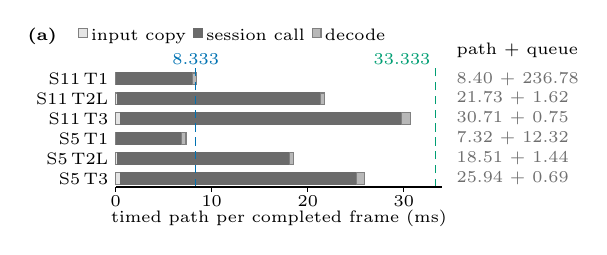
\begin{tikzpicture}[x=1pt,y=1pt,line width=0.4pt]
\definecolor{figblue}{RGB}{0,114,178}
\definecolor{figverm}{RGB}{213,94,0}
\definecolor{figgreen}{RGB}{0,158,115}
\definecolor{figgrey}{RGB}{110,110,110}
\providecommand{\fsix}{\fontsize{6}{7}\selectfont}
\draw[fill=black!10,draw=black!50] (32.00,79.00) rectangle (33.84,83.20);
\draw[fill=black!58,draw=black!58] (33.84,79.00) rectangle (118.94,83.20);
\draw[fill=black!28,draw=black!50] (118.94,79.00) rectangle (122.03,83.20);
\node[anchor=east,inner sep=0pt,font=\fsix] at (29.50,81.10) {S5\,T3};
\node[anchor=west,inner sep=0pt,font=\fsix,text=figgrey] at (155.00,81.10) {25.94 $+$ 0.69};
\draw[fill=black!10,draw=black!50] (32.00,86.20) rectangle (32.76,90.40);
\draw[fill=black!58,draw=black!58] (32.76,86.20) rectangle (94.89,90.40);
\draw[fill=black!28,draw=black!50] (94.89,86.20) rectangle (96.23,90.40);
\node[anchor=east,inner sep=0pt,font=\fsix] at (29.50,88.30) {S5\,T2L};
\node[anchor=west,inner sep=0pt,font=\fsix,text=figgrey] at (155.00,88.30) {18.51 $+$ 1.44};
\draw[fill=black!10,draw=black!50] (32.00,93.40) rectangle (32.42,97.60);
\draw[fill=black!58,draw=black!58] (32.42,93.40) rectangle (55.93,97.60);
\draw[fill=black!28,draw=black!50] (55.93,93.40) rectangle (57.42,97.60);
\node[anchor=east,inner sep=0pt,font=\fsix] at (29.50,95.50) {S5\,T1};
\node[anchor=west,inner sep=0pt,font=\fsix,text=figgrey] at (155.00,95.50) {7.32 $+$ 12.32};
\draw[fill=black!10,draw=black!50] (32.00,100.60) rectangle (33.82,104.80);
\draw[fill=black!58,draw=black!58] (33.82,100.60) rectangle (135.42,104.80);
\draw[fill=black!28,draw=black!50] (135.42,100.60) rectangle (138.57,104.80);
\node[anchor=east,inner sep=0pt,font=\fsix] at (29.50,102.70) {S11\,T3};
\node[anchor=west,inner sep=0pt,font=\fsix,text=figgrey] at (155.00,102.70) {30.71 $+$ 0.75};
\draw[fill=black!10,draw=black!50] (32.00,107.80) rectangle (32.65,112.00);
\draw[fill=black!58,draw=black!58] (32.65,107.80) rectangle (106.06,112.00);
\draw[fill=black!28,draw=black!50] (106.06,107.80) rectangle (107.43,112.00);
\node[anchor=east,inner sep=0pt,font=\fsix] at (29.50,109.90) {S11\,T2L};
\node[anchor=west,inner sep=0pt,font=\fsix,text=figgrey] at (155.00,109.90) {21.73 $+$ 1.62};
\draw[fill=black!10,draw=black!50] (32.00,115.00) rectangle (32.39,119.20);
\draw[fill=black!58,draw=black!58] (32.39,115.00) rectangle (59.63,119.20);
\draw[fill=black!28,draw=black!50] (59.63,115.00) rectangle (61.17,119.20);
\node[anchor=east,inner sep=0pt,font=\fsix] at (29.50,117.10) {S11\,T1};
\node[anchor=west,inner sep=0pt,font=\fsix,text=figgrey] at (155.00,117.10) {8.40 $+$ 236.78};
\draw[figblue,densely dashed] (60.92,78.00) -- (60.92,122.20);
\node[anchor=south,inner sep=1pt,font=\fsix,text=figblue] at (60.92,121.20) {8.333};
\draw[figgreen,densely dashed] (147.69,78.00) -- (147.69,122.20);
\node[anchor=south east,inner sep=1pt,font=\fsix,text=figgreen] at (146.89,121.20) {33.333};
\draw[draw=black] (32.00,78.00) -- (150.00,78.00);
\draw[draw=black] (32.00,78.00) -- (32.00,76.20);
\node[anchor=north,inner sep=1pt,font=\fsix] at (32.00,76.20) {0};
\draw[draw=black] (66.71,78.00) -- (66.71,76.20);
\node[anchor=north,inner sep=1pt,font=\fsix] at (66.71,76.20) {10};
\draw[draw=black] (101.41,78.00) -- (101.41,76.20);
\node[anchor=north,inner sep=1pt,font=\fsix] at (101.41,76.20) {20};
\draw[draw=black] (136.12,78.00) -- (136.12,76.20);
\node[anchor=north,inner sep=1pt,font=\fsix] at (136.12,76.20) {30};
\node[anchor=north,inner sep=0pt,font=\fsix] at (91.00,70.00) {timed path per completed frame (ms)};
\node[anchor=south west,inner sep=0pt,font=\fsix] at (155.00,124.70) {path $+$ queue};
\node[anchor=south west,inner sep=0pt,font=\fsix] at (0.0,129.20) {\textbf{(a)}

\
\ \tikz[baseline=-0.5ex]{\filldraw[fill=black!10,draw=black!50](0,0)rectangle(3.2pt,3.2pt);}\,input copy\ \tikz[baseline=-0.5ex]{\filldraw[fill=black!58,draw=black!58](0,0)rectangle(3.2pt,3.2pt);}\,session call\ \tikz[baseline=-0.5ex]{\filldraw[fill=black!28,draw=black!50](0,0)rectangle(3.2pt,3.2pt);}\,decode};
\end{tikzpicture}
